\section*{Parallel Speeedup and Efficiency}

The second task of exercise 1 was to parallelize a stencil-based Jacobi solver for the following 2D elliptic PDE problem:

\begin{gather*}
-\Delta u(x,y) + k^2 u(x,y) = k^2 u_p(x,y) \quad \text{with} \quad k=2\pi \\
\Omega = \left[ 0,1 \right] \times\left[ 0,1 \right] \\
u_p(x,y) = sin(2 \pi x ) sinh(2 \pi y) \\
u(0,y) = u(1,y) = u(x,0) = 0 \\
u(x,1) = sin(2 \pi x ) sinh(2\pi) 
\end{gather*}

The problem was discretized on a equidistant finite-difference grid with the above described Dirichlet boundary conditions.
The parallization was done by implementation of an \texttt{MPI}-based domain decomposition  in $x$-direction on $\Omega$.
Furthermore, the parallel speedup and the parallel efficiency where investigated for 4 different grid resolutions of the domain $\Omega$.
In order to obtain significant results for the timings, 100 iterations per settings were averaged.

\begin{figure}[ht]
    \centering
    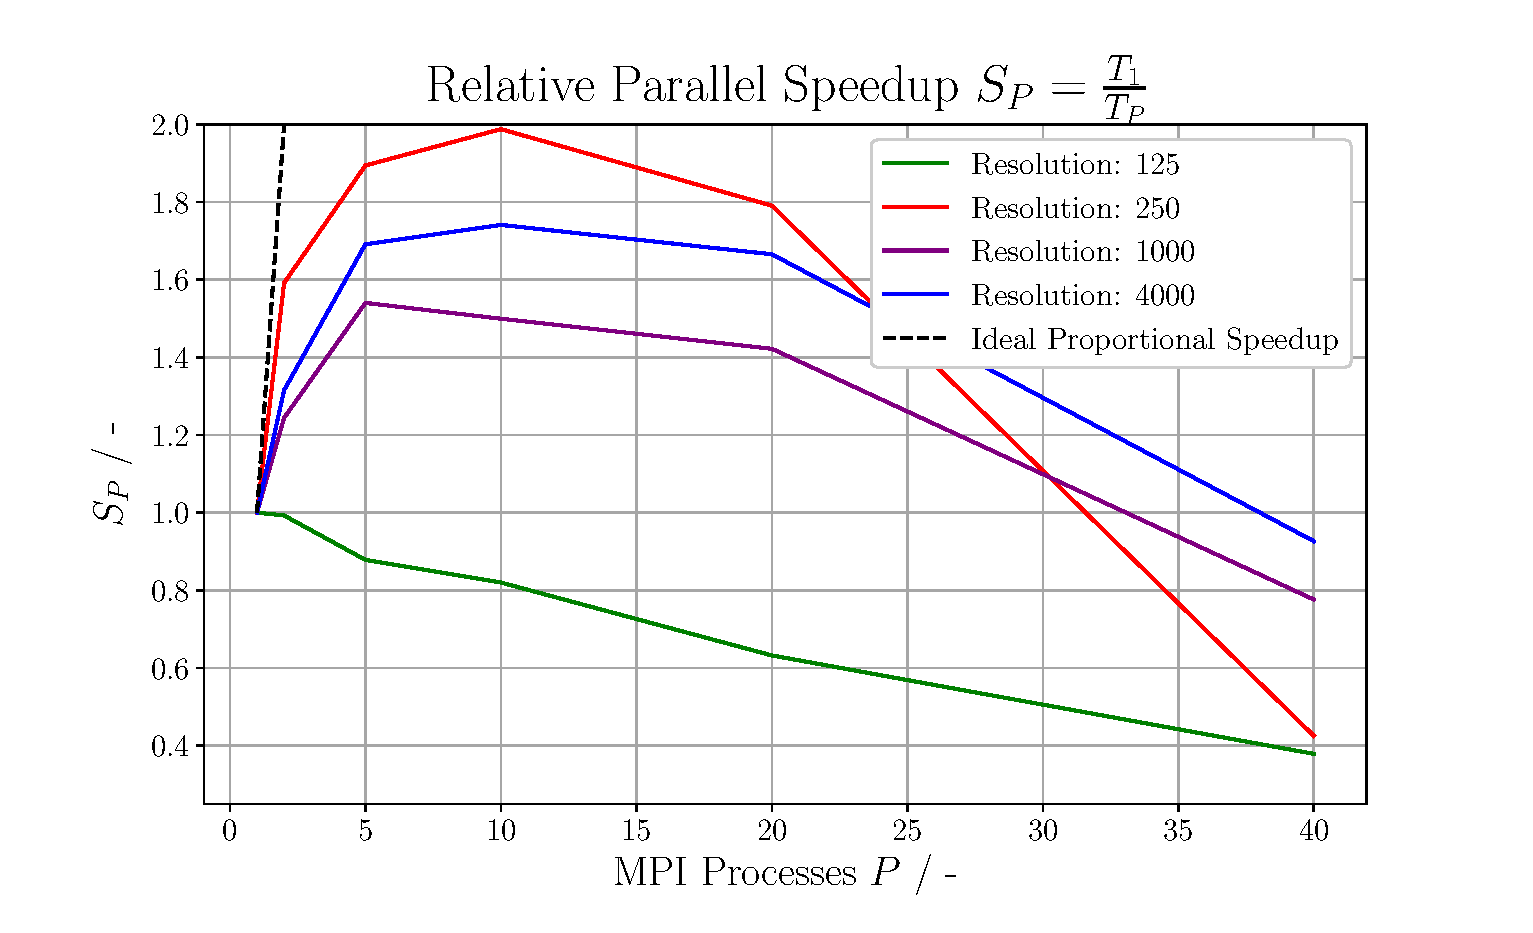
\includegraphics[width=1\textwidth]{figures/S_P_rel.eps}
	\caption{Parallel Speedup for 1D Decomposition of $\Omega$ with 1, 2, 5, 10, 20 and 40 Processes}
	\label{speedup_fig}
\end{figure}

For a grid resolution of 125, one can identify the dominance of the parallelization overhead in figure \ref*{speedup_fig} since it drops below 1 for 2 processes already.
The best speedup out of the 4 discretizations, was achieved by the 250 grid resolution (red graph in \ref*{speedup_fig}).
For 2 processes, said grid resolution lead to almost linear proportional speedup. Its maximum speedup for the chosen processes can be observed
at 10 processes with a speedup factor of almost 2. For 40 processes, one can observe the expected behaviour, where larger problems benefit from parallelization
and the largest problem has the highest speedup and the smallest problem the smallest speedup, which can also be observed in figure \ref*{efficiency_fig},
which is obvious since both figures stem from the same data.

\pagebreak

\begin{figure}[ht]
	\centering
    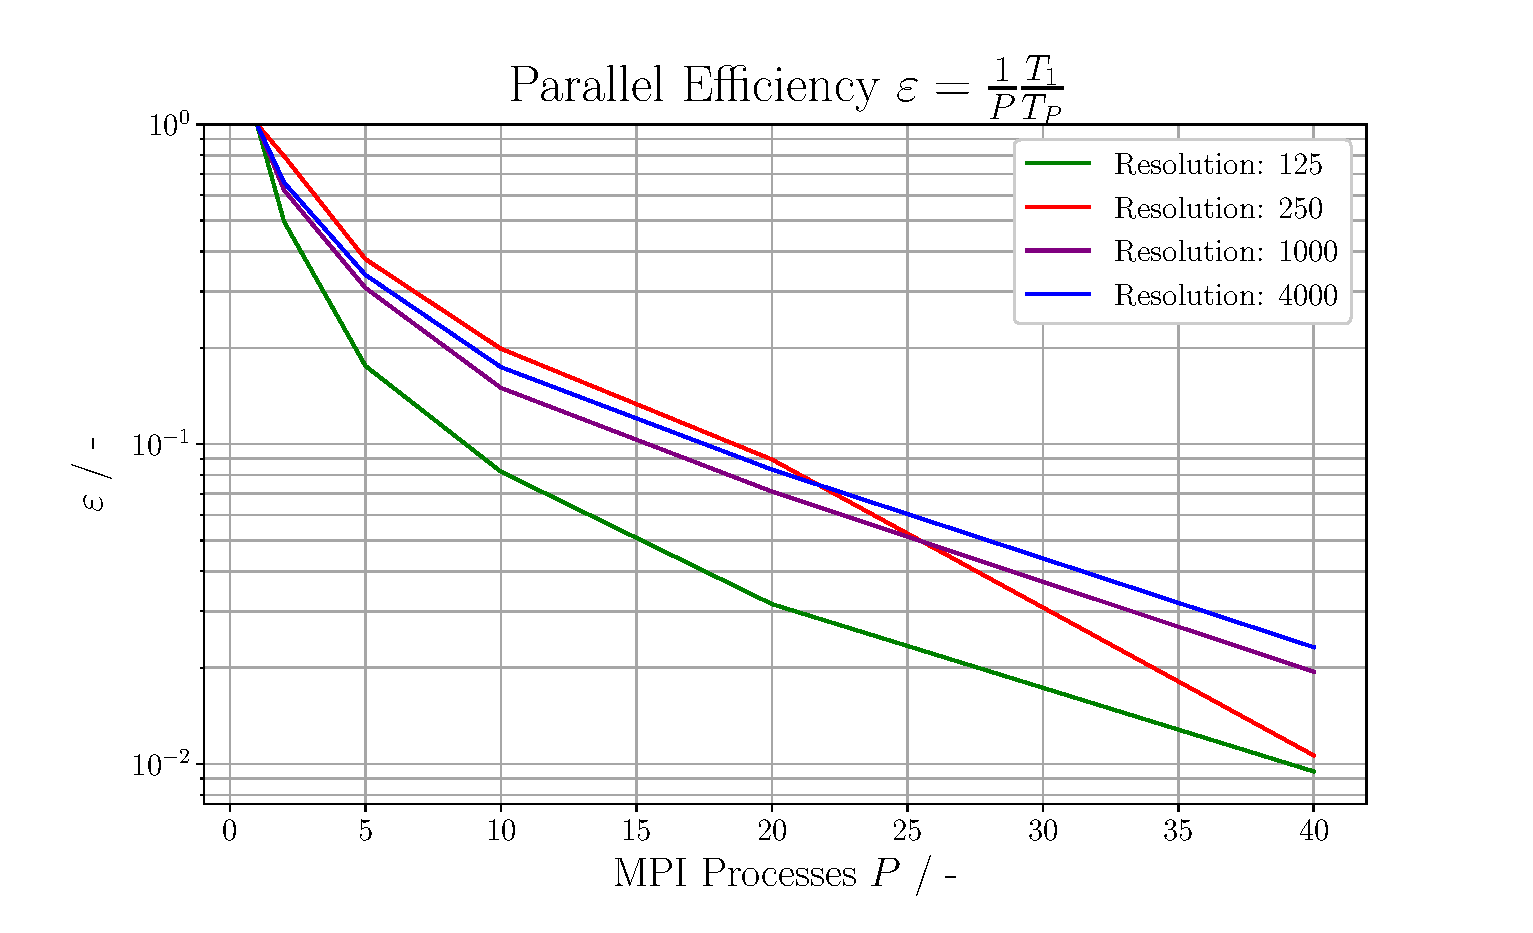
\includegraphics[width=1\textwidth]{figures/epsilon_semilogy.eps}
	\caption{Parallel Efficiency for 1D Decomposition of $\Omega$ with 1, 2, 5, 10, 20 and 40 Processes}
    \label{efficiency_fig}
\end{figure}

In figure \ref*{efficiency_fig} above, the parallel efficiency is shown over \texttt{MPI}-processes.
Visible is again the overhead dominance in the low grid resolution of 125, leading to the overall lowest parallel efficiency for the compared cases.
This overhead dominance leads to a significant efficiency drop for a grid resolution of 250 as well, but only for the jump from 20 to 40 \texttt{MPI} processes.
Again since speedup and efficiency stem from the same data, the large problem size of grid resolution 4000 benefits from parallelization and
has therefore the best parallel efficieny out of the 4 cases.



